\begin{figure}[h!]
    \centering{
        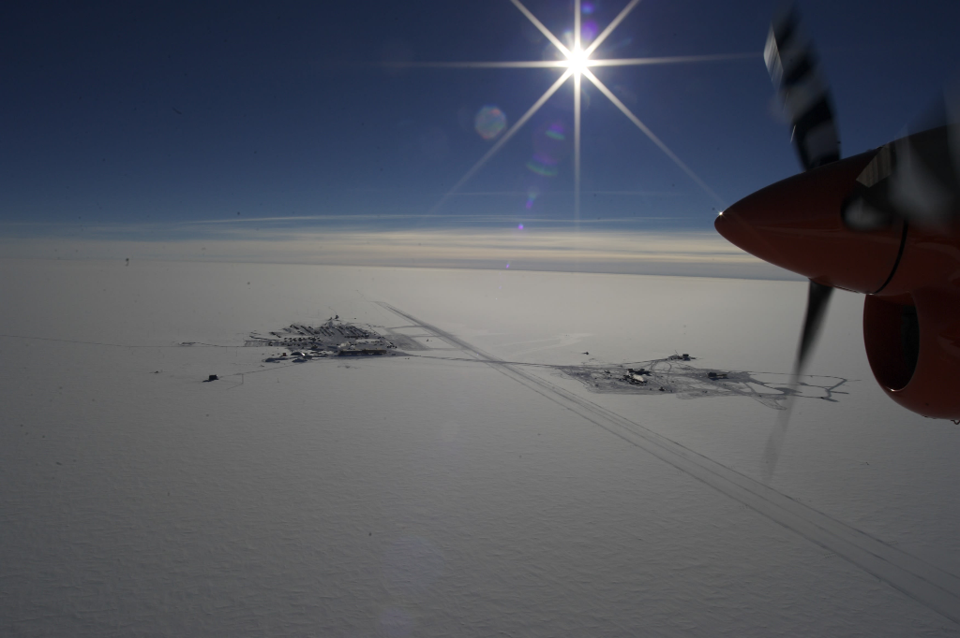
\includegraphics[clip, trim=3cm 3.5cm 2cm 0cm, scale=0.8]{figures/ic3/IC3_aboveground.png}
    }
    \caption{IceCube Neutrino observatory at the South Pole. Image from \todo{cite where you got this from}.}
    \label{fig:IC3_atPole}
\end{figure}

Located at the South Pole, the IceCube Neutrino Observatory is a pivotal instrument for neutrino astronomy.
IceCube's primary function is the detection and analysis of elusive, high-energy neutrinos.
These neutrinos carry information from the most energetic and distant cosmic phenomena.
The observatory uses thousands of digital optical modules embedded in a cubic kilometer of Antarctic ice to detect Cherenkov radiation.
This radiation occurs when neutrinos interact with the ice, revealing their origin and energy.

IceCube is a critical component in the multi-messenger astrophysics toolkit, especially in the search for dark matter and beyond standard model (BSM) astrophysical processes.
The observatory's analysis of neutrino signals enhances our understanding of the universe by correlating these signals with other cosmic messengers, including electromagnetic, gravitational waves, and cosmic rays.

The following sections will discuss the observatory's design, data acquisition, event reconstruction methodologies, and its significance in observing the Northern Sky.
These details will underscore IceCube's role in advancing our understanding of the cosmos through data-driven insights.

%-----------------------------------------------------------------------------------%
\section{The Detector}
%-----------------------------------------------------------------------------------%

The IceCube Neutrino Observatory is embedded within a cubic kilometer of Antarctic ice at the South Pole.
IceCube's modules are designed to detect neutrinos through Cherenkov radiation emitted during neutrino interactions with the ice.
It comprises 5160 Digital Optical Modules (DOMs), arranged across 86 strings that span depths of 1450 m to 2450 m beneath the surface.
This arrangement allows IceCube to capture high-energy neutrinos across a broad neutrino spectrum.

%$$$$$$$$$$$$$$$$$$$$$$$$$$$$$$$$$$$$$$$$$$$$$$$$$$$$$$$$$$$$$$$$$$$$$$$$$$$$$$$$$$$%
\subsection{Hardware and Construction}
%$$$$$$$$$$$$$$$$$$$$$$$$$$$$$$$$$$$$$$$$$$$$$$$$$$$$$$$$$$$$$$$$$$$$$$$$$$$$$$$$$$$%

\begin{figure}
    \centering{
        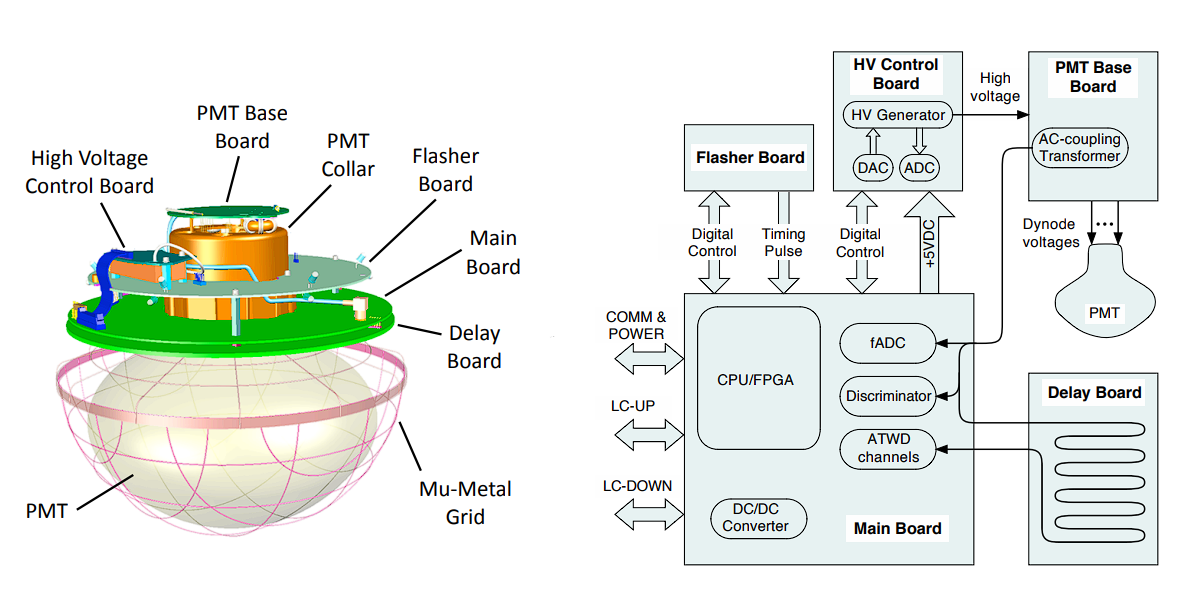
\includegraphics[scale=0.5]{figures/ic3/DOM.png}
    }
    \caption{\todo{pasted} Components of the DOM, showing mechanical layout (left) and functional connections (right). Figure from \cite{IC3_thedetector}}
    \label{fig:DOM}
\end{figure}

Digital Optical Modules (DOMs) are at the core of IceCube’s detection technology, each encased in a glass sphere to withstand deep-ice pressures.
A DOM features a 10-inch photomultiplier tube (PMT) for Cherenkov light detection, a high-voltage power supply for the PMT, and a Main Board for signal digitization and timestamping.
An LED Flasher Board is included for calibration purposes, assisting in verifying DOM responses and measuring ice optical properties.
The DOMs are deployed along cables on strings in a hexagonal grid pattern, which spans a cubic kilometer.
Strings are placed with 125 meters of horizontal spacing, and DOMs are vertically separated by 17 meters on each string, chosen to optimize detection capability for neutrinos within the teraelectronvolt (TeV) to petaelectronvolt (PeV) energy range.

DeepCore and IceTop, additional components of IceCube, extend its research capabilities.
DeepCore, with its denser array of DOMs, targets lower energy neutrinos for studies such as neutrino oscillations and dark matter.
IceTop, situated at the ice surface, measures cosmic rays, contributing data that complement the neutrino observations from below the ice.

\begin{figure}
    \centering{
        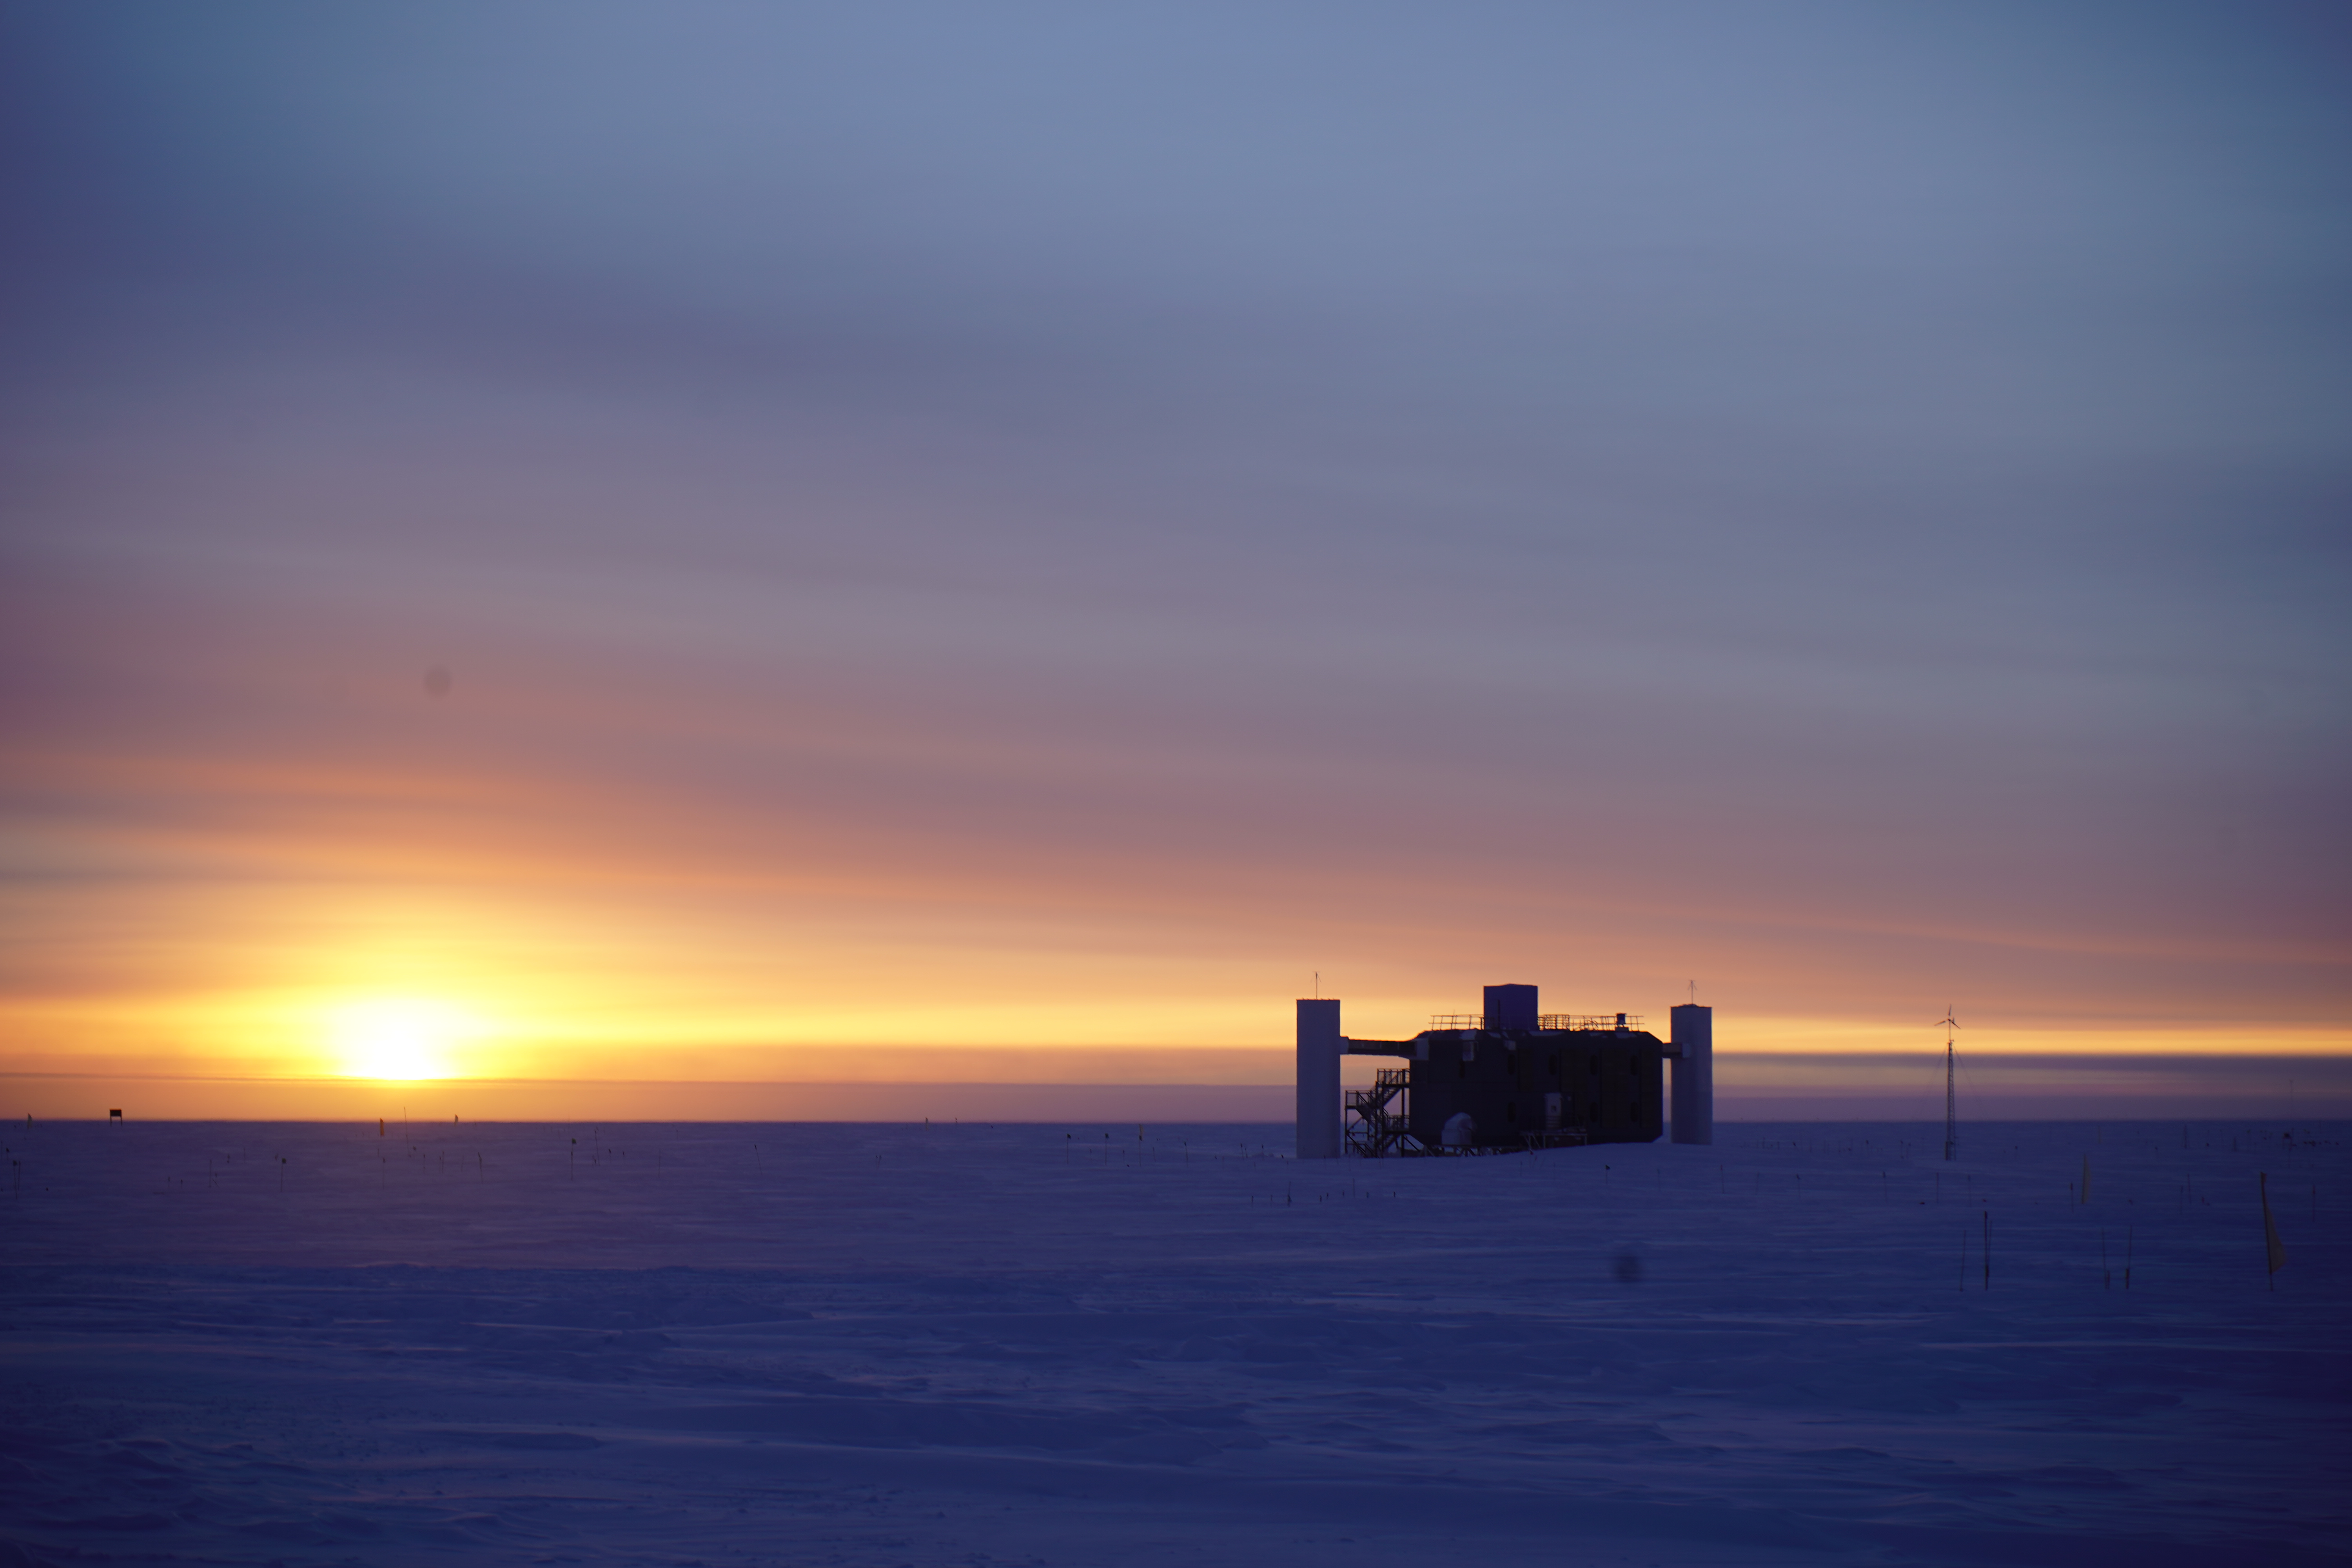
\includegraphics[scale=0.37]{figures/ic3/ICL.JPG}
    }\caption{ICL. Picture from \cite{IceCube_SPGallery}.}
    \label{fig:ICL}
\end{figure}

The central hub for IceCube's operations is the IceCube Laboratory (ICL), situated at the surface at the center of the array.
This facility houses the servers and computers responsible for data acquisition and online filtering, connected to the DOMs via cables routed up from beneath the ice \cite{IC3_thedetector}.
The ICL plays a crucial role in managing the data flow from the ice, ensuring continuous operation and data integrity.
It is designed to maintain optimal conditions for its electronic equipment, including temperature control and protection against electromagnetic interference, which is vital for the accurate processing and analysis of the collected data \cite{IC3_thedetector}.


%$$$$$$$$$$$$$$$$$$$$$$$$$$$$$$$$$$$$$$$$$$$$$$$$$$$$$$$$$$$$$$$$$$$$$$$$$$$$$$$$$$$%
\subsection{Data Acquisition}
%$$$$$$$$$$$$$$$$$$$$$$$$$$$$$$$$$$$$$$$$$$$$$$$$$$$$$$$$$$$$$$$$$$$$$$$$$$$$$$$$$$$%

\begin{figure}
    \centering{
        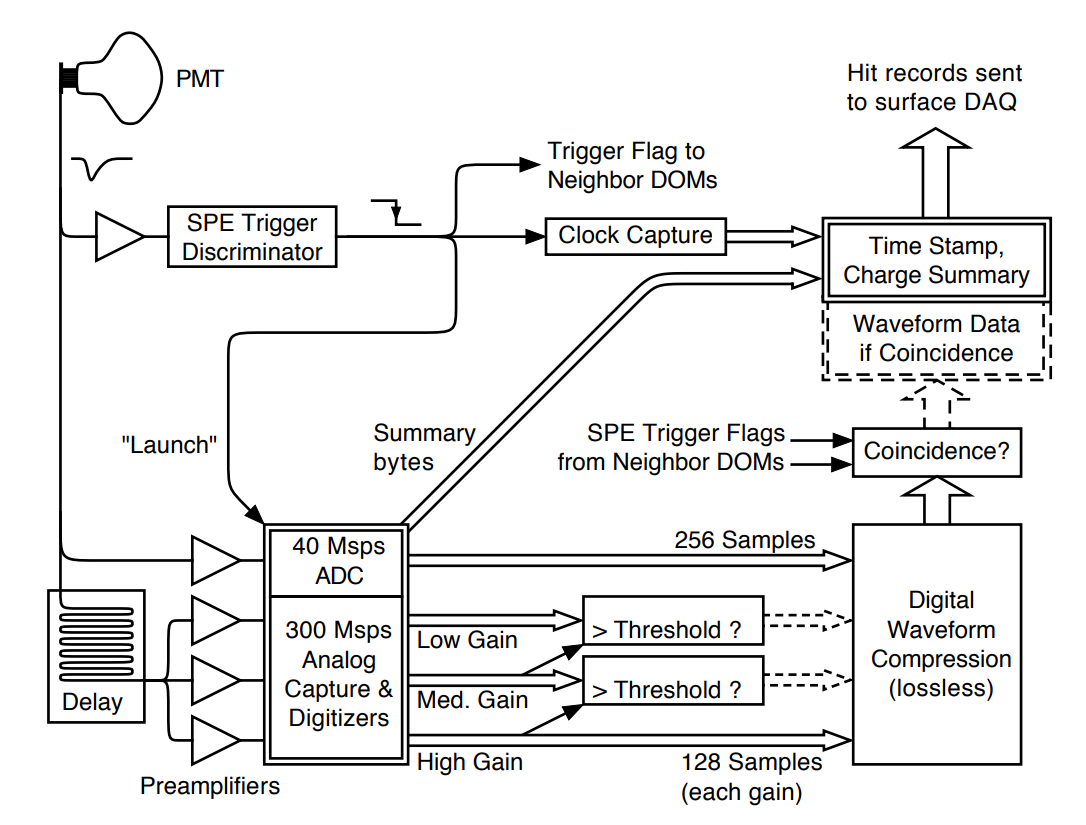
\includegraphics[scale=0.4]{figures/ic3/IC3_dataflow.png}
    }
    \caption{\todo{Copied} Data flow diagram for recording and processing of PMT waveforms in the DOM to form “Hit Records" that are sent to the surface DAQ computers. As shown by dashes, full waveform data are only included when neighbor DOMs report time-coincident signals above the SPE discriminator threshold. Additionally, data from low-gain channels are omitted for waveforms that are within range of higher-gain channels.}
    \label{fig:IC3_dataflow}
\end{figure}

The data acquisition process in the IceCube Neutrino Observatory starts when a photomultiplier tube (PMT) within a Digital Optical Module (DOM), distributed between 1450 m and 2450 m beneath the ice, detects light surpassing a threshold of 0.25 photoelectrons.
The importance of the information transmitted to the surface computers depends on the detection of signals by neighboring DOMs within a microsecond window.
Isolated signals prompt a Soft Local Coincidence (SLC) response, transmitting only a timestamp and a charge summary.
In contrast, signals detected by neighboring DOMs initiate a Hard Local Coincidence (HLC), resulting in the full waveform being compressed and sent along with the timestamp and charge summary to the IceCube Laboratory (ICL), located at the surface at the center of the array \cite{IC3_thedetector}.

Achieving uniform timing across DOMs is essential for accurate event reconstruction.
Each DOM's independent clock undergoes a rigorous calibration process to synchronize with the ICL's clocks, with the times further translated to Universal Coordinated Time (UTC).
This calibration is critical, involving continuous pulses sent between the DOMs and the ICL to adjust the waveforms by subtracting the common baseline and applying the gain.
This step is vital for the precise interpretation of the collected data \cite{IC3_thedetector}.

Within the ICL, the Data Acquisition (DAQ) system employs various trigger algorithms to discern neutrino events from the vast majority of DOM hits caused by dark noise.
One such mechanism, the Simple Multiplicity Trigger (SMT), requires a specific number of HLC hits within a brief timeframe to recognize a series of hits as an event.
This approach is pivotal for identifying sequences of detections likely resulting from neutrino interactions \cite{IC3_thedetector}.

Further refining the observatory's data, the Processing and Filtering (PnF) system, also housed within the ICL, applies around 25 different filters after initial event detection.
Each filter is designed for specific physics analyses, significantly managing the observatory's data throughput by focusing on scientifically valuable information.
The system employs filters like the Muon Track Filter to isolate high-quality track events crucial for neutrino source identification, the Shower Event Filter to select events with large energy deposits indicative of neutrino interactions, and the High-Charge Filter to highlight events with extensive photoelectron deposits, pointing to high-energy astrophysical neutrinos.
These filters ensure that the data prepared for further analysis and transmission to researchers in the Northern Hemisphere contains the most significant scientific insights \cite{IC3_thedetector}.

The operational control of the observatory, maintained by the LiveControl system within the ICL, oversees the DAQ and PnF systems.
It handles the initiation and conclusion of data-taking runs and maintains a database of operational parameters.
Alerting operators to any deviations from expected conditions, this system is crucial for ensuring the observatory operates within its optimal parameters, highlighting the integrated effort required to manage and analyze the vast data generated by the IceCube Neutrino Observatory \cite{IC3_thedetector}.

%-----------------------------------------------------------------------------------%
\section{Event Reconstruction}
%-----------------------------------------------------------------------------------%
Event Reconstruction within the IceCube Neutrino Observatory transforms signals captured by Digital Optical Modules into quantifiable scientific insights, clarifying the origin, trajectory, and strength of interacting neutrinos. This complex process is pivotal for interpreting signals as either originating from celestial neutrino sources or other phenomena, enabling a broad spectrum of astrophysical and particle physics research.

%$$$$$$$$$$$$$$$$$$$$$$$$$$$$$$$$$$$$$$$$$$$$$$$$$$$$$$$$$$$$$$$$$$$$$$$$$$$$$$$$$$$%
\subsection{Tracks and Cascades}
%$$$$$$$$$$$$$$$$$$$$$$$$$$$$$$$$$$$$$$$$$$$$$$$$$$$$$$$$$$$$$$$$$$$$$$$$$$$$$$$$$$$%

\tmpfig{Track}
\tmpfig{Cascade}
\tmpfig{Double Bang}

In IceCube's detection landscape, events manifest primarily as either tracks or cascades, contingent on the neutrino flavor and the nature of its interaction with the ice.

Tracks emerge from charged-current interactions involving muon (μ) neutrinos.
These events are characterized by the production of a muon, which, due to its relatively large mass compared to electrons, can travel extensive distances through the ice, exceeding kilometers.
This extensive travel path is marked by a continuous emission of Cherenkov light, forming a distinct, elongated track in the detector's observational field.
The angular deviation between the incoming μ neutrino and the produced muon is notably slight, tapering to near 0.3$^\circ$ at energies surpassing a teraelectronvolt (TeV), thereby allowing the trajectory of the muon to closely approximate the incident neutrino's path.
Such precision affords angular resolutions finer than 1$^\circ$ for neutrinos with energies in the TeV range and beyond, facilitating the accurate determination of their cosmic origins.

Cascades are indicative of both neutral-current interactions across all neutrino flavors and charged-current interactions involving electron (e) or tau (τ) neutrinos.
Unlike tracks, cascades result in a more localized explosion of Cherenkov radiation, rendering a nearly spherical light pattern due to the rapid dissipation of energy by the produced particles.
This diffusion creates a distinct event signature but sacrifices the directional clarity afforded by track events.
Despite the isotropic nature of cascades leading to broader angular uncertainties—typically around 15$^\circ$ — they excel in providing precise energy measurements, with resolutions reaching as tight as 15\%, due to the contained nature of the energy deposition.

A theoretical event type, the double-bang event, posited for τ neutrinos interacting via charged-current mechanisms at energies above 1 PeV, would display as two distinct cascades within the detector.
This signature arises from the initial interaction and subsequent decay of the τ lepton over a discernible distance, offering a unique marker for high-energy τ neutrino detection.
While IceCube has yet to identify such an event, its potential discovery would significantly advance our understanding of neutrino physics.

Delineating events into tracks, cascades, and the theoretical double-bangs is essential for extracting meaningful data from the myriad of interactions within IceCube.
This categorization underpins the observatory's ability to probe the universe's extremities, offering insights into the enigmatic sources of high-energy neutrinos and the fundamental properties governing their behavior.

%$$$$$$$$$$$$$$$$$$$$$$$$$$$$$$$$$$$$$$$$$$$$$$$$$$$$$$$$$$$$$$$$$$$$$$$$$$$$$$$$$$$%
\subsection{Angle}
%$$$$$$$$$$$$$$$$$$$$$$$$$$$$$$$$$$$$$$$$$$$$$$$$$$$$$$$$$$$$$$$$$$$$$$$$$$$$$$$$$$$%

%$$$$$$$$$$$$$$$$$$$$$$$$$$$$$$$$$$$$$$$$$$$$$$$$$$$$$$$$$$$$$$$$$$$$$$$$$$$$$$$$$$$%
\subsection{Energy}
%$$$$$$$$$$$$$$$$$$$$$$$$$$$$$$$$$$$$$$$$$$$$$$$$$$$$$$$$$$$$$$$$$$$$$$$$$$$$$$$$$$$%

%-----------------------------------------------------------------------------------%
\section{Background}
%-----------------------------------------------------------------------------------%

%-----------------------------------------------------------------------------------%
\section{North Sky Tracks}
%-----------------------------------------------------------------------------------%
